\documentclass[11pt]{article}

%% Language and font encodings
\usepackage[english]{babel}
\usepackage[utf8x]{inputenc}
\usepackage[T1]{fontenc}

\usepackage{amsmath,mathtools,amssymb}


%%%%%%%%%%%%%%%%%%%
% aliases
%%%%%%%%%%%%%%%%%%%

\newcommand{\T}[2]{\prescript{#1}{}{\bfT}_{#2}}
% \newcommand{\Th}[2]{\prescript{#1}{}{\widehat T}_{#2}}  % ?
\newcommand{\Tm}[2]{\prescript{#1}{}{\widetilde{\bfT}}_{#2}}
\newcommand{\Rot}[2]{\prescript{#1}{}{\bfR}_{#2}}
\newcommand{\Rotm}[2]{\prescript{#1}{}{\widetilde{\bfR}}_{#2}}
\newcommand{\noise}{\bfn}

\newcommand{\posiv}[1]{\underline{\bfp}_{#1}}
\newcommand{\posi}[2]{\prescript{#1}{}{\bfp}_{#2}}
\newcommand{\posim}[2]{\prescript{#1}{}{\widetilde{\bfp}}_{#2}}
\newcommand{\velv}[1]{\underline{\bfv}_{#1}}
\newcommand{\vel}[2]{\prescript{#1}{}{\bfv}_{#2}}
\newcommand{\velm}[2]{\prescript{#1}{}{\widetilde{\bfv}}_{#2}}
\newcommand{\accv}[1]{\underline{\bfa}_{#1}}
\newcommand{\acc}[2]{\prescript{#1}{}{\bfa}_{#2}}
\newcommand{\accm}[2]{\prescript{#1}{}{\widetilde{\bfa}}_{#2}}
\newcommand{\angvelv}[1]{\underline{\pmb{\omega}}_{#1}}
\newcommand{\angvel}[2]{\prescript{#1}{}{\pmb{\omega}}_{#2}}
\newcommand{\angvelm}[2]{\prescript{#1}{}{\widetilde{\pmb{\omega}}}_{#2}}
\newcommand{\forcev}[1]{\underline{\bff}_{#1}}
\newcommand{\force}[2]{\prescript{#1}{}{\bff}_{#2}}
\newcommand{\forcem}[2]{\prescript{#1}{}{\widetilde{\bff}}_{#2}}
\newcommand{\torquev}[1]{\underline{\pmb{\tau}}_{#1}}
\newcommand{\torque}[2]{\prescript{#1}{}{\pmb{\tau}}_{#2}}
\newcommand{\torquem}[2]{\prescript{#1}{}{\widetilde{\pmb{\tau}}}_{#2}}

\newcommand{\AM}{\mathcal{L}}
\newcommand{\AMv}{\underline{\mathcal{L}}}
\newcommand{\COM}{\bfc}
\newcommand{\COMv}{\underline{\bfc}}

\newcommand{\grav}{\bfg}
\newcommand{\gravv}{\underline{\bfg}}

\newcommand{\Gaussian}[2]{\mathcal{N}({#1},{#2})}

%%%%%%%%%%%%%%%%%%%

\usepackage{customCommands} % Joan Sola's macros


\topmargin -.5in
\textheight 9in
\oddsidemargin -.25in
\evensidemargin -.25in
\textwidth 7in

\begin{document}

\author{Médéric Fourmy}
\title{Humanoid robot state estimation}
\maketitle

\section{Camera extrinsics calibration using Apriltag and kinematics}
\subsection{Motivation}
A camera is placed at an unknown location in a humanoid robot head. We want to estimate the camera pose with respect to the end of the kinematic chain of the robot: the neck joint frame.
The robot's feet are stuck on the ground and we move its torso so that it takes a look around a scene with fixed Apriltags. We want to fuse both kinematic and Apriltag information to estimate the neck camera transformation $\T{K}{C}$.

\subsection{Problem formulation}
The problem is formulated as a factor graph in which keyframes states are poses of a frame from the robot kinematic frame that has a static transform with regard to the camera (the neck joint frame). The camera calibration problem can be expressed as a factor graph represented in figure \ref{fig:factorgraph}. We will estimate simultaneously the neck frame trajectory and the apriltag locations in the scene. As the feet are fixed, we can choose the foot frame as an absolute frame and express both the trajectory and apriltag poses in it.

Then to types of factors constrain the problem.

\subsubsection*{Apriltag factor}
It is a 6D binary factor that depends on the ith keyframe pose, jth landmark pose and camera extrinsics:

% $$
% r(\T{F}{K_i}, \T{F}{L_j}, \T{K}{C}) = Log_{SE(3)}(\T{C}{L_j}^{-1}  \T{K}{C}^{-1}\T{F}{K_i}^{-1}\T{F}{L_j}) ~ \in ~ \mathrm{}{}{R}^6
% $$


\subsubsection*{Kinematic unary factor (Wolf Pose3D)}
6D unary factor constraining the ith keyframe pose:

\begin{equation*}
e(\T{F}{K_i}) = Log_{SE(3)}(\Tm{F}{K_i}^{-1} \T{F}{K_i})    
\end{equation*}



\section{Kinematic odometry}
The goal of this section is to find a way to use kinematics measurements of the pose of the body frame relative to its contacts with the environment as well as feet force torque sensors to design a relative pose factor (Odom3D in wolf jargon) between body frames at different timestamp. Force torque sensors will be used as a way to determine the contact states, that is to say whether or not the contact remains static from one timestamp to an other: for example a support foot could be slipping on the ground, tilting on an edge etc.
Special care will be given to the computation of the different measurements covariances that depend on the contact states, kinematic inconsistencies or flexibilities, encoders errors...

\subsection{Odom3D factor}
An 3D odometry factor constraints two poses through a relative pose measurement. In our case the, poses we which to constraints are the absolute pose of the body frame from timestamps $t_{i-1}$ and $t_{i}$: $\T{W}{B_{i-1}}$ and $\T{W}{B_i}$. The residual of this factor is defined as $\bfr^2 = ||\bfe(\T{W}{B_{i-1}}, \T{W}{B_i})||^2_{\bfQ_{i/i-1}}$
 with:
 
 \begin{equation*}
 \bfe(\T{W}{B_{i-1}}, \T{W}{B_i}) =  Log_{SE(3)}(
 \T{W}{B_{i-1}}^{-1}
 \T{W}{B_i}
 \T{B_{i-1}}{B_i}^{-1}
 )     
 \end{equation*} 

\subsection{Single foot in support phase}
Let's begin with a simplified case of a humanoid robot in support phase on a single foot.
We want to measure the relative pose of the base frame at times $t_{i-1}$ and $t_i$. This pose can be decomposed in three poses: 

\begin{equation*}
\Tm{B_{i-1}}{B_i} = 
\Tm{B_{i-1}}{F_{i-1}}
\Tm{F_{i-1}}{F_{i}} 
\Tm{F_{i}}{B_i}     
\end{equation*}

A few comments on the different quantities. $ \Tm{B_{i-1}}{F_{i-1}} $ and $ \Tm{F_{i}}{B_i} $ are kinematic measurements made at time $t_{i-1}$ and $t_{i}$ respectively that are affected by the encoder noises, kinematic model inconsistencies and robot flexibilities (TODO). However, we have no direct measurement over $\Tm{F_{i-1}}{F_{i}}$. One way to proceed is to assume that $\Tm{F_{i-1}}{F_{i}}=\bfI_4$ and assign it a covariance based on the foot force/torque sensors measurements (TODO inspired by Thomas F.). Then these three measurements are composed to get a covariance on $\Tm{B_{i-1}}{B_i}$ using first order approximation or as explained in \cite{barfoot2014associating}.

\subsection{Fusing multiple contacts}
In the case of humanoid locomotion we have 2 pose measurements of the same quantity using both foot. 

One easier way to implement it is to include both measurements as separate Odom3D factors in the graph. Measurements with covariance too high (foot flying, slipping or tilting) can be plainly discarded using an upper threshold on the covariance determinant.

Another option is to fuse in an optimal way the pose measurements based on there covariances. This would result in a single factor and is the problem tackled in section IV of \cite{barfoot2014associating}. This enables handling an arbitrary number of contacts with reduced computational burden.


\section{Center of mass estimation}
\subsection{Blibliography}
- Stephens
- Xinjilefu
- Bloesch student
- ...

\subsection{End effector force/torque sensors factor}
We will here develop a factor graph for the estimation of Center of mass (Com) position, velocity and angular momentum (AM) expressed at the COM using force/torque measurements at the end effectors of a humanoid robot. A relation between these quantities will be derived through the Newton-Euler equations. It will be shown that by expressing these equation at the COM a chosen inertial frame $W$, as it is usually done, we have to include the position, orientation and velocity of a body reference frame, quantities that are not supposed to be known in advance. 
Therefore, we define a state vector: 

\begin{equation*}
\bfx = [\posi{W}{WB}, \vel{W}{WB}, \Rot{W}{B}, \posi{W}{WC}, \vel{W}{WC}, \prescript{W}{}{\AM}_{c}] 
\triangleq 
[\bfp, \bfv, \Rot{}{}, \COM, \dot{\COM}, \AM_c] 
\end{equation*}

where $B$ and $C$ correspond to the frame/frame origin (appropriately) of the robot body and the COM. Notations of the state blocks are simplified in order to make it easier to differentiate them with other terms in the subsequent equations.

With this formulation, the factor will also include IMU measurements so that the control/measurement vector writes: 

\begin{equation*}
% \bfu = [\prescript{B}{}{\bfa}_B, \prescript{B}{}{\bf\omega}_B, \prescript{L}{}{\bff}_l~\prescript{L}{}{\bf\tau_l}]
\bfu = [\forcem{L}{l}~\torquem{L}{l}]
\end{equation*}

for $l \in 1..N$, with N number of force sensors and L the frame attached to this sensor (that we will drop subsequently for shorter notations).
By integrating measurements from $t_i$ to $t_j$, we wish to derive a factor constraining $\bfx_i$ and $\bfx_j$.

\subsubsection{Force/torque sensors measurements model}
Each end effector $l \in 1..N$ is equipped with a sensor measuring forces $\bff \in \mathrm{R}^3$ and pure torques $\tau \in \mathrm{R}^3$ along the three orthogonal axis of its reference frame. The measurements are assumed to be corrupted by a zero mean Gaussian noise:

\begin{equation}
\begin{split}
    \forcem{}{l} = \force{L}{l} + \noise_f~~~~~\noise_f \sim \mathcal{N}(O,Q_{\bff})
    \\
    \torquem{}{l} = \torque{L}{l} + \noise_{\tau} ~~~~~ \noise_{\tau} \sim \mathcal{N}(O,Q_{\tau})
\end{split}
\end{equation} 

\textbf{Unknown biases} drifting with time could potentially be added and estimated (TBD). 
In all equations, unless otherwise specified \textbf{kinematic measurements} (depending on ($q$ and $\dot{q}$) are considered to be exact. We should consider adding them in the measurement vector in a second time to account for encoder noises or flexibilities.
For lighter notation we will subsequently omit the measurement frame of references noting simply \(\forcem{}{l}\) and \(\torquem{}{l}\) for force and torque measurement values.


\subsubsection{COM state dynamics driven by force/torque sensors}
The Newton-Euler equations at the COM with respect to an inertial frame can be written:

\begin{equation}
\begin{split}
m\ddot{\COMv}&= m\gravv + \sum_l \forcev{l}
\\
\dot{\AMv}_c&= \sum_l \torquev{l} + ( \posiv{WL} - \COMv) \times \forcev{l} 
\end{split}
\label{eq:NewtonEuler}
\end{equation}

where \(\posiv{L} \) is the position vector of each end effector in the inertial frame.

Incorporating the measurements model in equation \ref{eq:NewtonEuler} and expressing it in the world frame \(W\), we derive the equations:

\begin{equation}
\begin{split}
m\ddot{\COM}&= 
m\bfg + \Rot{}{} \sum_l \Rot{B}{L}(q) (\forcem{}{l} - \noise_f) 
\\
\dot{\AM}_c&= 
\sum_l \Rot{}{}\Rot{B}{L}(q)(\torquem{}{l} - \noise_{\tau}) + (\Rot{}{} \posi{B}{CL}(q)) \times (\Rot{}{}\Rot{B}{L}(q)(\forcem{}{l} - \noise_f))
\\
&= \sum_l \Rot{}{}\Rot{B}{L}(q)(\torquem{}{l} - \noise_{\tau}) + \Rot{}{}( \posi{B}{BL}(q) - (\posim{B}{BC}(q)) -  \bfb_{p} - \noise_p) \times (\Rot{B}{L}(q)(\forcem{}{l} - \noise_f))
\end{split}
\end{equation}

It can be reformulated as the state-space model equation on the COM related variables \( \frac{d\bfx_c}{dt}= f(\bfx_c, \bfu, t)$ with $\bfx_c = [\COM, \dot{\COM}, \AM_c]\):

\begin{equation}
\begin{split}
\frac{d\COM}{dt} &= \dot{\COM} 
\\
\frac{d\dot{\bfc}}{dt}&= \bfg + \frac{1}{m} \Rot{}{} \sum_l \Rot{B}{L}(q) (\forcem{}{l} - \noise_f) 
\\
\frac{d\AM_c}{dt}&= \Rot{}{} \sum_l \Rot{B}{L}(q)(\torquem{}{l} - \noise_{\tau}) + (\posi{B}{BL}(q) - (\posim{B}{BC}(q)) -  \bfb_{p} - \noise_p) \times (\Rot{B}{L}(q)(\forcem{}{l} - \noise_f))
\end{split}
\label{eq:COMContinuous}
\end{equation}

We will consider the quantity $\posi{b}{BC}$  as a measurement disturbed by a Gaussian noise and a time varying bias considered constant during pre-integration period. 
 
\begin{equation}
\posim{B}{BC} = \posi{B}{BC}(q) + \bfb_{p} + \noise_p 
\end{equation}

All other terms computed through direct kinematics are in first hand considered as exact values but are in fact corrupted by (supposedly) gaussian noise due to encoder noise, flexibilities, model errors...

\begin{equation}
\begin{split}
\posim{A}{AB} = \posi{A}{AB}(q) + \noise_p ~~~ \noise_p \sim \Gaussian{0}{Q_p}, ~ Q_p \in \mathrm{R}^{3\times 3} 
\\
\Rotm{A}{B} = \Rot{A}{B}(q) Exp(\phi) ~~~ \phi \sim \Gaussian{0}{Q_{\phi}}, ~ Q_{\phi} \in \mathrm{R}^{3\times 3}
\end{split}
\end{equation}
 
Considering again the angular momentum theorem expressed in W, this leads to:
 
\begin{equation}
\begin{split}
    \frac{d\AM_c}{dt} &= \sum_l \Rot{}{}\Rot{B}{L}(q)(\torquem{}{l} - \noise_{\tau}) + (\Rot{}{} \posi{B}{CL}(q)) \times (\Rot{}{}\Rot{B}{L}(q)(\forcem{}{l} - \noise_f))
\\
&= \sum_l \Rot{}{}\Rot{B}{L}(q)(\torquem{}{l} - \noise_{\tau}) + \Rot{}{}( \posi{B}{BL}(q) - (\posim{B}{BC} -  \bfb_{p} - \noise_p) \times (\Rot{B}{L}(q)(\forcem{}{l} - \noise_f))
\end{split}
\end{equation}


We now need to discretize this continuous system to define factors between successive times. We integrate \ref{eq:COMContinuous} between 2 consecutive measurements ($t_k$ and $t_{k+1}$ $\Delta t = t_{k} - t_{k-1}$)  We use a simple first order approximation (forward Euler) which consists in assuming a zero order hold. We may also add a second order term for the com position since we have measurements on its acceleration.

\begin{equation}
\begin{split}
\COM^{k+1} &= \COM^{k} + \dot{\COM}^{k} \Delta t 
+ \dfrac{1}{2}(\bfg + \frac{1}{m} \Rot{}{}^{k} \sum_l \Rot{B}{L}(q^{k}) (\forcem{}{l}^{k} - \noise_f^{k})) \Delta t^2
\\
\dot{\COM}^{k+1}&= \dot{\COM}^{k} + (\bfg + \frac{1}{m} \Rot{}{}^{k} \sum_l \Rot{B}{L}(q^{k}) (\forcem{}{l}^{k} - \noise_f^{k})) \Delta t 
\\
\AM_c^{k+1} &= \AM_c^{k} +  ( 
\Rot{}{}^{k}\sum_l \Rot{B}{L}(q^{k})(\torquem{}{l}^{k} - \noise_{\tau}^{k}) + (\posi{B}{BL}(q^k) - \posim{B}{BC}^k + \bfb_{p}^k + \noise_p^k) \times \Rot{B}{L}(q^{k})(\forcem{}{l}^{k} - \noise_f^{k}) 
) \Delta t
\end{split}
\label{eq:COMDiscrete}
\end{equation}

with discrete noise quantities distributed according to \( \mathcal{N}(O,\frac{Q}{\Delta t}) \), \(Q\) being the corresponding continuous covariance.


\subsubsection{Factor between successive measurements}
Based on equations \ref{eq:COMDiscrete}, we will define the 3 functions \(g_1\), \(g_2\) and \(g_3\) specifying which variables they depend on:

\begin{equation}
\begin{split}
\COM^{k+1} - \COM^{k} &=  g_1(\dot{\COM}^{k}, \Rot{}{}^{k}, \noise_f^{k})
\\
\dot{\COM}^{k+1} - \dot{\COM}^{k} &= g_2(\Rot{}{}^{k}, \noise_f^{k}) 
\\
\AM_c^{k+1} - \AM_c^{k} &= g_3(\Rot{}{}^{k}, \bfb_{p}^k, \noise_p^k, \noise_f^{k}, \noise_\tau^{k})
\end{split}
\end{equation}

In order to propagate the measurement covariances, we need to derive the related jacobians.

\subsubsection{Pre-integrated COM factor}
Solved for COM position and velocity but AM is less obvious (different possibilities are presented). Adding measurements between 2 arbitrary timestamps \(t_i\) and \(t_j\) with \(\Delta t_{ij} \triangleq t_j - t_i\), we get the equations:

\begin{equation}
\begin{split}
\COM^{j} - \COM^{i} &= \sum_{k=i}^{j-1} \Big[ 
\dot{\COM}^{k} \Delta t 
+ \dfrac{1}{2}\bfg \Delta t^2 + \frac{1}{2m} \Rot{}{}^{k} \sum_l \Rot{B}{L}(q^{k}) (\forcem{}{l}^{k} - \noise_f^{k})\Delta t^2 \Big]
\\
\dot{\COM}^{j} - \dot{\COM}^{i} &= \sum_{k=i}^{j-1} \Big[ 
\bfg + \frac{1}{m} \Rot{}{}^{k} \sum_l \Rot{B}{L}(q^{k}) (\forcem{}{l}^{k} - \noise_f^{k}) \Big] \Delta t 
\\
\AM_c^{j} - \AM_c^{i} &=  \sum_{k=i}^{j-1} \Rot{}{}^{k} \Big[ 
\sum_l \Rot{B}{L}(q^{k-1}) (\torquem{}{l}^{k} - \noise_{\tau}^{k} - (\forcem{}{l}^{k} - \noise_f^{k}) \times (\posi{B}{BL}(q^k) - \posim{B}{BC}^k + \bfb_{p}^k + \noise_p^k) \Big]  \Delta t
\end{split}
\label{eq:COMij}
\end{equation}


It is then possible to define a "delta" quantity depending only on the measurements relating the com position, com velocity and Angular Momentum at \(t_i\) and \(t_j\):

\begin{equation}
\begin{split}
    \Delta \COM_{ik} &\triangleq \Rot{}{}^{i,T} (\COM^j - \COM^i - \vel{}{}^i \Delta t_{ij} - \frac{1}{2}\grav \Delta t_{ij}^2) 
    \\
    &= \sum_{k=i}^{j-1} \Big[ \Delta \dot{\COM}_{ik} \Delta t + \frac{1}{2m} \Delta R_{ik} \sum_l \Rot{B}{L}(q^{k}) (\forcem{}{l}^{k} - \noise_f^{k}) \Delta t^2 \Big]
\\
    \Delta \dot{\COM}_{ik} &\triangleq \Rot{}{}^{i,T} (\dot{\COM}^{k} - \dot{\COM}^{i} - \bfg \Delta t_{ik})
\\
    &= \sum_{k=i}^{j-1} \frac{1}{m} \Delta R_{ik} \sum_l \Rot{B}{L}(q^{k}) (\forcem{}{l}^{k} - \noise_f^{k}) \Delta t 
\\
    \Delta \AM_{ik} &\triangleq \Rot{}{}^{i,T} (\AM_c^{j} - \AM_c^{i})
\\
     &=  \sum_{k=i}^{j-1} \Delta R_{ik} \Big[ 
    \sum_l \Rot{B}{L}(q^{k-1}) (\torquem{}{l}^{k} - \noise_{\tau}^{k} - (\forcem{}{l}^{k} - \noise_f^{k}) \times (\posi{B}{BL}(q^k) - \posim{B}{BC}^k + \bfb_{p}^k + \noise_p^k) \Big]  \Delta t
\end{split}
\label{eq:COMPreint}
\end{equation}

We can then define a recursive scheme to retrieve measurement values and a covariance propagation scheme akin to the IMU pre-integration framework. 
Difficulties that might come up during implementation:

\begin{itemize}
    \item Angular momentum and force/torque measurements are not recovered at the same frequency -> consider a constant delta for the slowest one?
    \item COM preint factor noise is correlated with the IMU one since the gyro noise is propagated through it as well.
\end{itemize}



\subsection{COM differential kinematics}

\begin{itemize}
    \item \( \angvel{}{WB} \): angular velocity vector describing the rotation rate of \textbf{frame B with respect to the observer inertial frame}
    \item \( \bfI(q) \): inertia matrix of the robot expressed at the COM
    \item \( \AM_q (q,\dot{q}) \): Angular momentum of the limbs ("gesticulation")
\end{itemize}

\begin{equation}
\begin{split}
\dot{\COMv} &= \angvelv{B} \times \posiv{BC}(q) + \velv{B} + \velv{BC}(q,\dot{q}) 
\\
\AMv_c &= \bfI(q) \angvelv{B} + \AMv_q (q,\dot{q})   
\end{split}
\end{equation}

Measurement model:
\begin{align}
    \angvelm{}{} = \angvel{B}{WB} + \bfb_{\omega} + \noise_{\omega}
\end{align}

Differential kinematics expressed in $W$ with measurement models included and rearranged terms:

\begin{equation}
\begin{split}
\dot{\COM} &= \vel{}{} + (\Rot{}{}(\angvelm{B}{B} - \bfb_{\omega} - \noise_{\omega})) \times (\Rot{}{}\posim{B}{BC}(q)) + \Rot{}{}\velm{B}{BC}(q,\dot{q}) 
\\
&= \vel{}{} + \Rot{}{}((\angvelm{B}{B} - \bfb_{\omega} - \noise_{\omega}) \times \posi{B}{BC}(q) + \vel{B}{BC}(q,\dot{q}))
\\
\AM_c &= \Rot{}{}(\bfI(q) (\angvelm{B}{B} - \bfb_{\omega} - \noise_{\omega}) + \AM_q (q,\dot{q}))
\end{split}
\end{equation}

\subsection{COM kinematics}
Very simply, the COM position (in the world frame) can be recovered from kinematic measurements and the current robot body frame pose estimation as:

\begin{equation}
    \COM = \Rot{}{} \posi{B}{BC}(q) + \posi{}{}
\end{equation}

However, great care should be given defining a measurement model for \(\posi{B}{BC}(q)\). This data is potentially corrupted by 3 factors:
\begin{itemize}
    \item encoder noise
    \item errors in the inertial/kinematic model of the robot
    \item structural flexibilities
\end{itemize}

While the first term could be regarded as a Gaussian perturbation, the two others are clearly bias terms that depend strongly on robot configuration and the dynamics/phases of the movement.  

As a first approach, let's consider a simple additive Gaussian noise model:

\begin{equation}
    \posim{B}{BC}(q) = \posi{B}{BC}(q) + \noise_p ~~~~~~ \noise_p \sim \Gaussian{O}{Q_p}
\end{equation}

Hence we get:

\begin{equation}
    \posim{B}{BC}(q) = \Rot{}{}^T(\COM - \posi{}{}) + \noise_p
\end{equation}

which directly defines a tertiary factor between the pose (R,p) of the robot and the COM position. This is a 3D factor constraining 3 3D vectors which means it is greatly undetermined: the factor graph has to include factor making, by themselves, the robot pose observable.



\subsection{TODO}
\begin{itemize}
    \item Add external force/moment to the estimated state? 
\end{itemize}


\begin{figure}[ht]
    \centering
    % 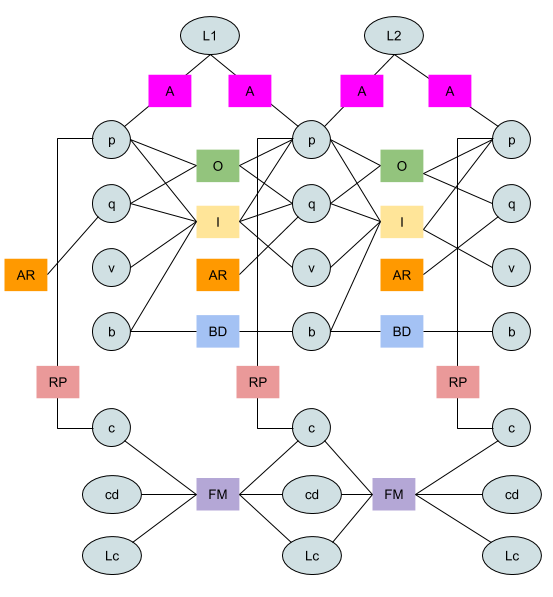
\includegraphics[width=0.7\linewidth]{IMU-Apriltag-Kinematics-Com.png}
    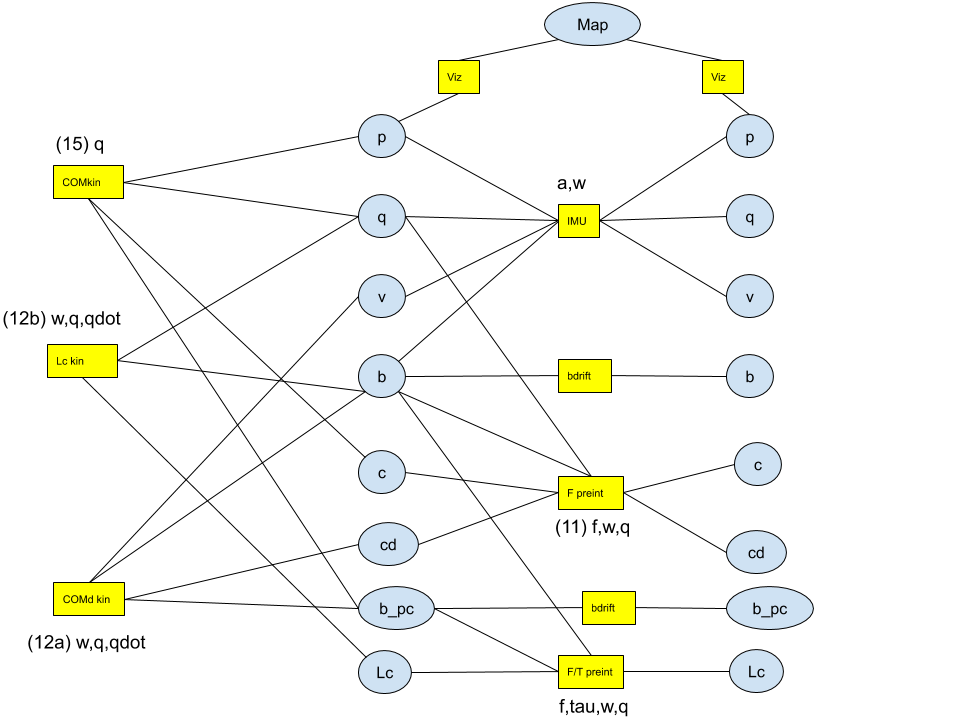
\includegraphics[width=1\linewidth]{HumanoidStateFactorGraph.png}
    % \caption{Factor graph representation of the simultaneous estimation of the robot state and COM state. Gray circles represent variables with from top to bottom Li: landmarks, p: robot position, q: robot orientation, v: robot velocity, b: IMU biases, c: COM position in foot frame, cd: COM velocity in foot frame, Lc: system angular momentum in foot frame. Constraints are represented as squares with A: Apriltag, O: odometry using forward kinematics, I: IMU, AR: absolute orientation, BD: bias drift, RP: relative position of the COM wrt. the robot reference frame, FM: force and moment measurements integration.}
    % \caption{Latest version at https://docs.google.com/drawings/d/1XQ80bcXe--4V49n_bDHHNxId_9YTiQ_YTVO0kwxaypA}
    \label{fig:my_label}
\end{figure}





\section{Notations}
\begin{itemize}
    \item $\T{Y}{X}$: transformation SE(3) transformation so that $\prescript{Y}{}{v}=\T{Y}{X}\prescript{X}{}{v}$
    \item $\Tm{Y}{X}$: transformation measurement
    \item $C$: camera frame
    \item $K$: frame corresponding to the end of robot kinematic chain 
    \item $F$: one of the foot frame 
\end{itemize}

\begin{figure}[ht]
\begin{minipage}[c]{.46\linewidth}
    \centering
    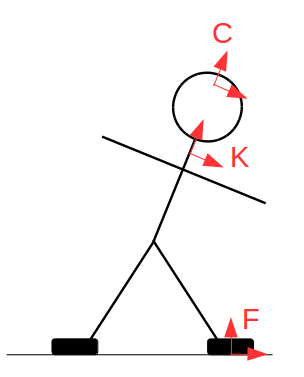
\includegraphics[width=0.6\linewidth]{robot_sketch.png}
    \label{fig:sketch}
    \caption{Frames diagram}
\end{minipage} \hfill
\begin{minipage}[c]{.46\linewidth}
    \centering
    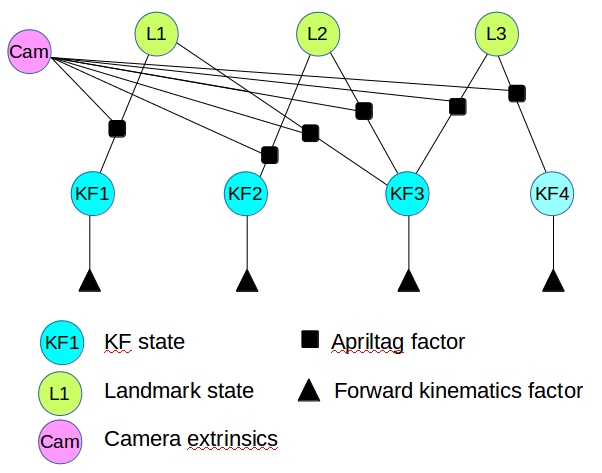
\includegraphics[width=\linewidth]{cam_extrinsics_factor_graph.png}
    \label{fig:factorgraph}
    \caption{Extrinsics calibration factor graph}
\end{minipage}
\end{figure}









\section{Annexes}
\subsection{IMU pre-integration Delta derivation (Forster's)}
\subsubsection{Integration of pqv between distant timestamps}
State to estimate:

\begin{equation*}
\bfx = [\posi{W}{WB}, \vel{W}{WB}, \Rot{W}{B}, \bfb_{\angvel{}{}}, \bfb_{\bfa}]
\triangleq 
[\bfp, \bfv, \Rot{}{}, \bfb_{\angvel{}{}}, \bfb_{\bfa}] 
\end{equation*}

Continuous state space equations:

\begin{equation*}
\frac{d\posi{}{}}{dt} = \vel{}{}  ~~~~ \frac{d\vel{}{}}{dt} = \acc{W}{WB} ~~~~ \frac{d\Rot{}{}}{dt} = \Rot{}{} \angvel{B}{WB} 
\end{equation*}

Measurement model:

\begin{equation*}
\begin{split}
\angvelm{}{} &= \angvel{B}{WB} + \bfb_{\angvel{}{}} + \noise_{\angvel{}{}} 
\\
\accm{}{}    &= \acc{B}{WB} + \bfb_{\acc{}{}} + \noise_{\acc{}{}} 
\end{split}
\end{equation*}


Taylor type, zero hold on measurement integration during $dt = t_k - t_{k-1}$:

\begin{equation*}
\begin{split}
\Rot{}{}^{k+1}  &= \Rot{}{}^{k}Exp((\angvelm{}{}^k - \bfb_{\angvel{}{}^k} - \noise_{\angvel{}{}^k})dt)
\\
\vel{}{}^{k+1}  &= \vel{}{}^{k} + \grav dt + \Rot{}{}^{k}(\accm{}{}^k - \bfb_{\acc{}{}^k} - \noise_{\acc{}{}^k})dt
\\
\posi{}{}^{k+1} &= \posi{}{}^{k} + \vel{}{}^{k}dt + \frac{1}{2}\grav dt^2 
+ \frac{1}{2}\Rot{}{}^{k}(\accm{}{}^k - \bfb_{\acc{}{}^k} - \noise_{\acc{}{}^k})dt^2
\end{split}
\end{equation*}


Summing from $k=i$ to $k=j-1$:

\begin{equation}
\begin{split}
\Rot{}{}^{j}  &= \Rot{}{}^{i} \prod_{k=i}^{j-1} Exp((\angvelm{}{}^k - \bfb_{\angvel{}{}^k} - \noise_{\angvel{}{}^k})dt)
\\
\vel{}{}^{j}  &= \vel{}{}^{i} + \sum_{k=i}^{j-1} \Big[\grav dt + \Rot{}{}^{k}(\accm{}{}^k - \bfb_{\acc{}{}^k} - \noise_{\acc{}{}^k})dt \Big]
\\
\posi{}{}^{j} &= \posi{}{}^{i} + \sum_{k=i}^{j-1} \Big[\vel{}{}^{k}dt + \frac{1}{2}\grav dt^2 
+ \frac{1}{2}\Rot{}{}^{k}(\accm{}{}^k - \bfb_{\acc{}{}^k} - \noise_{\acc{}{}^k})dt^2 \Big]
\end{split}
\label{eq:IMUIntij}
\end{equation}

\subsubsection{Pre-interation formulas}
\textit{Quick def:} The goal is to define quantities that represent the movement of B relative to the time i so that those can be computed once and for all (except for bias adjustment, see later) by integrating measurements between i and j. We will proceed by rearranging the terms of \ref{eq:IMUIntij} to define these so called "delta quantities".

The rotation one is easy to get, multiplying by $\Rot{}{}^{i,T}$:
\begin{equation}
    \Delta R_{ij} \triangleq \Rot{}{}^{i,T} \Rot{}{}^{j} = \prod_{k=i}^{j-1} Exp((\angvelm{}{}^k - \bfb_{\angvel{}{}^k} - \noise_{\angvel{}{}^k})dt)
    \label{eq:IMUDeltaR}
\end{equation}

The velocity is as well quite easy, by defining $\Delta t_ij \triangleq \sum_{k=i}^{j-1} dt = (j-i)dt = (j - i)dt$:
\begin{equation}
    \Delta v_{ij} \triangleq \Rot{}{}^{i,T} (\vel{}{j} - \vel{}{i} - g \Delta t_{ij}) 
    = \prod_{k=i}^{j-1} \Delta R_{ik} Exp((\accm{}{}^k - \bfb_{\acc{}{}^k} - \noise_{\acc{}{}^k})dt)
    \label{eq:IMUDeltav}
\end{equation}

The position delta requires more calculations. First, inject equation \ref{eq:IMUDeltav} in the position equation of \ref{eq:IMUIntij} then rearrange and reorder the terms.

\begin{equation}
\begin{split}
\posi{}{}^{j} - \posi{}{}^{i} &= \sum_{k=i}^{j-1} \Big[
(\vel{}{}^i + \grav \Delta t_{ik} + \Rot{}{}^i \Delta v_{ik})dt 
+ \frac{1}{2}\grav dt^2 + \frac{1}{2}\Rot{}{}^{k}(\accm{}{}^k - \bfb_{\acc{}{}^k} - \noise_{\acc{}{}^k})dt^2 \Big]
\\
&= \vel{}{}^i \Delta t_{ij} + 
\grav\sum_{k=i}^{j-1} \Delta t_{ik} dt + \frac{1}{2}\grav \sum_{k=i}^{j-1} dt^2 +
\Rot{}{}^i\sum_{k=i}^{j-1} \Big[\Delta v_{ik}dt +  \frac{1}{2} \Delta R_{ik} (\accm{}{}^k - \bfb_{\acc{}{}^k} - \noise_{\acc{}{}^k})dt^2 \Big]
\\
&= \vel{}{}^i \Delta t_{ij} + 
\grav \sum_{k=i}^{j-1}dt (\Delta t_{ik} + \frac{1}{2}dt^2) +
\Rot{}{}^i\sum_{k=i}^{j-1} \Big[\Delta v_{ik}dt +  \frac{1}{2} \Delta R_{ik} (\accm{}{}^k - \bfb_{\acc{}{}^k} - \noise_{\acc{}{}^k})dt^2 \Big]
\end{split}
\end{equation}

We will simplify the gravity term that we will call $\mathcal{G}t_{ij}$. Noting that:

\begin{equation*}
    \sum_{k=i}^{j-1}k = \sum_{k=1}^{j-1}k - \sum_{k=1}^{i-1}k = \frac{j(j-1)}{2} - \frac{i(i-1)}{2} 
\end{equation*}

we can deduce that:

\begin{equation*}
\begin{split}
\mathcal{G}t_{ij} 
&= dt \sum_{k=i}^{j-1}(\Delta t_{ik} + \frac{1}{2}dt) = dt \sum_{k=i}^{j-1}((k -i)dt + \frac{1}{2}dt)
\\
&= dt \Big[ \sum_{k=i}^{j-1} k dt - i(j-i)dt + \frac{1}{2}\Delta t_{ij}  \Big] 
\\
&= dt \Big[ \frac{dt}{2} (j(j-1) - i(i-1) - 2i(j-1)) + \frac{1}{2}\Delta t_{ij} \Big] 
\\
&= dt \Big[ \frac{dt}{2} (i^2 - 2ij + j^2 + i - j) + \frac{1}{2}\Delta t_{ij} \Big] 
\\
&= dt \Big[ \frac{1}{2} (j-i)^2dt - \frac{1}{2}(j - i)dt + \frac{1}{2}\Delta t_{ij} \Big]
\\
&= \frac{1}{2} (j-i)^2dt^2 = \frac{1}{2} \Delta t_{ij}^2
\end{split}
\end{equation*}
Multiplying by $\Rot{}{}^{i,T}$ and reordering the terms, we can finally define a position delta quantity:

\begin{equation}
    \Delta p_{ij} \triangleq \Rot{}{}^{i,T}(\posi{}{}^j - \posi{}{}^i - \vel{}{}^i \Delta t_{ij} - \frac{1}{2} \grav \Delta t_{ij}^2) = \sum_{k=i}^{j-1} \Big[\Delta v_{ik}dt +  \frac{1}{2} \Delta R_{ik} (\accm{}{}^k - \bfb_{\acc{}{}^k} - \noise_{\acc{}{}^k})dt^2 \Big]
\end{equation}


\subsection{COM estimation random notes}

Instead of using the biased kinematic measurement $\posim{B}{BC}$, we can 

\begin{equation}
\begin{split}
\frac{d\AM_c}{dt}&= \sum_l \Rot{}{}\Rot{B}{L}(q)(\torquem{}{l} - \noise_{\tau}) + (\bfp +
\Rot{}{}\posi{B}{BL}(q) - \COM)) \times \Rot{}{}\Rot{B}{L}(q)(\forcem{}{l} - \noise_f)
\end{split}
\label{eq:AMContinuousRandomNotes}
\end{equation}

First order discretization of \ref{eq:AMContinuousRandomNotes} gives:

\begin{equation}
\begin{split}
\AM_c^{k+1} &= \AM_c^{k} +  ( 
\sum_l \Rot{}{}^{k}\Rot{B}{L}(q^{k})(\torquem{}{l}^{k} - \noise_{\tau}^{k}) + (\bfp^{k-1} +
\Rot{}{}^{k}\posi{B}{BL}(q^{k}) - \COM^{k})) \times \Rot{}{}^{k}\Rot{B}{L}(q^{k})(\forcem{}{l}^{k} - \noise_f^{k}) 
) \Delta t
\end{split}
\end{equation}



Adding measurements between 2 arbitrary timestamps \(t_i\) and \(t_j\) with \(\Delta t_{ij} \triangleq t_j - t_i\), we get the equations:

\begin{equation}
\begin{split}
\AM_c^{j} - \AM_c^{i} &=  \sum_{k=i}^{j-1} \Big[ 
\sum_l \Rot{B}{L}(q^{k-1}) (\torquem{}{l}^{k} - \noise_{\tau}^{k} - (\forcem{}{l}^{k} - \noise_f^{k}) \times (\bfp^{k} + \Rot{}{}^{k}\posi{B}{BL}(q^{k}) - \COM^{k})) \Big]  \Delta t
\end{split}
\end{equation}


for which preintegration equations are not obvious (in fact, they likely do not exist).



We can also derive the angular momentum equations in the inertial frame attached to one of the extremities in contact (the one that we trust the most maybe). We will only write the case where only one of the extremities is in contact: \(l*\).

\begin{equation}
\begin{split}
    \frac{d \prescript{L*}{}{\AM}_c}{dt} &=
    (\torquem{}{l} - \noise_{\tau}) + \posi{L*}{CL*}(q) \times (\forcem{}{l*} - \noise_f)
    \\
    &= (\torquem{}{l} - \noise_{\tau}) + (\Rot{L*}{B}(q)\Rot{}{}^T(\bfp - \COM) + \posi{L*}{BL*}(q)) \times (\forcem{}{l*} - \noise_f)
\end{split}
\end{equation}
 
but again this leads to untangled equations that cannot be pre-integrated.


\bibliography{biblio}
\bibliographystyle{plainnat}







\end{document}






